% !TEX root = ../main.tex

\section{Background}
\label{section:background}

We introduce the terminology, notation, and prior mathematical formulation of solutions for FIMPUL problems.

The \emph{Full-Instance}, \emph{Multi-label Prediction for Unknown Label counts} (FIMPUL) learning task has three key concepts.
First, \emph{multi-label learning} refers to the possibility that one example is attributed more than one label~\cite{multilabelMethods}.
Second, the term \emph{full-instance} should be understood in contrast to \emph{multi-instance} learning~\citep[e.g.,][]{multiInstance,multiInstanceMultiLabel}, for which it is considered natural to first segment an image, text or sound before performing prediction on each of the segments. In contrast, for full-instance learning problems, we cannot assume that there is an obvious or unique way to segment an instance so that the prediction problem can be decided based on that segment.
Third, the concept of \emph{unknown label counts} illustrates the case where the number of labels is unknown a priori for each example. Our proposed smooth surrogate of the F1 score allows to balance the tasks of label prediction and label count into one.

In the following sections, we will first introduce the notion of the smooth confusion matrix and in particular sigmoidF1.
Next, we briefly characterize existing families of solutions to FIMPUL problems.
They can be divided into two groups, \emph{fit-data-to-algorithm} solutions (a.k.a. \emph{problem tranformation}) and \emph{fit-algorithm-to-data} solutions (a.k.a.\ \emph{algorithm adaptation})~\cite{multilabelReview, multilabelReview2}. These will be discussed in \S\ref{section:background:fitdata} and \S\ref{section:background:fitalgorithm} respectively, followed by discussing shortcomings of these solutions in \S\ref{section:background:limitations} and proposing a new solution framework in \S\ref{section:background:solution}.
In Section~\ref{section:method}, we then fully detail a particular instance of this framework.

\subsection{Fit-data-to-algorithm solutions} 
\label{section:background:fitdata}
Briefly, in the case of \emph{fit-data-to-algorithm}, cross-entropy losses are used at training time and thresholding is done at inference time. 

More formally, we define a learning algorithm that maps inputs to outputs given a set of hyperparameters \(\mathcal{F}(\cdot ; \Theta): \mathcal{X} \rightarrow \mathcal{Y}\). For the purpose of fit-data-to-algorithm,
we define \(\mathcal{L}_{\text {multiclass}}\), a class of loss functions that
minimize predictions in relative terms. Binary cross-entropy, logistic regression and their
variants, such as focal loss or hinge loss are common choices when it comes to
multiclass prediction. Note that minimizing binary cross-entropy is equivalent to maximizing for log-likelihood
\cite[Section 4.3.4]{Bishop}. 
Cross-entropy loss can be formulated as
\(\mathcal{L}_{\text {CE}}=-\sum \log \left(p_{i}\right)\). 
More generally, the fit-data-to-algorithm formulation amounts to minimizing the loss on a class of neural networks, such that
%
\begin{equation}
\underset{\mathcal{L}_{\text {multiclass}}} {\min} \mathcal{F}\left(\cdot ;
\Theta; \mathcal{L}_{\text {multiclass}} (\mathbf{y}, \hat{\mathbf{y}})
¨bcon\right),
\end{equation}
%

This class of loss functions is particularly useful for multi-class unilabel predictions, when we can select top-1 label predictions, or multiclass multilabel predictions with known amount of labels $k_i$ per example/document $i$, when we can select the top-k. Note that one common approach in fit-data-to-algorithm is to establish a hierarchical structure in labels. This way, one can constrain the algorithm to learn only 1 or $k$ labels per group in the hierarchy. For example, DBPedia\footnote{\url{https://wiki.dbpedia.org/develop/datasets/latest-core-dataset-releases} \todo{replace with cite?}} establishes a hierarchical structure in Wikipedia infoboxes\footnote{\url{https://en.wikipedia.org/wiki/Help:Infobox} \daan{I do not think we need. a footnote here.}} and is commonly used to finetune state-of-the-art NLP models~\citep[see, e.g.,][]{XLNet, ULMFit}.

For many real world problems and datasets reducing the problem to top-k selection or establishing a hierarchical structure is an oversimplification, especially when classes are not mutually exclusive. Besides the four datasets we use for our experiments, we mention others in the related work section.

\subsection{Fit-algorithm-to-data solutions}
\label{section:background:fitalgorithm}
In the case of \emph{fit-algorithm-to-data} solutions, elements of the learning algorithm are changed to deal with non-mutually exclusive classes. Such elements can be the back propagation algorithm or the summation of losses from different learning tasks.
The aim \daan{Always? Or is this the most common way of approaching this? Or our formalization of either one?} is to both obtain\daan{or "optimize for both"?} a propensity of each label being true and a prediction of the number of true labels:
%
\begin{equation}
\underset{\mathcal{L}_{\text {multiclass}}, \mathcal{L}_{\text {count}}}
{\min} \mathcal{F}\left(\cdot ; \Theta; \mathcal{L}_{\text {multiclass}}
(\mathbf{y}, \hat{\mathbf{y}}) + \lambda \mathcal{L}_{\text {count}}
(\mathbf{n}, \hat{\mathbf{n}})\right),
\end{equation}
%
where \(n_i = \sum_j \mathds{1}_{\mathbf{y_i^j} = 1}\) is the count of
positive labels per example. We thus impose a regularize the multiclass loss with the accuracy of retrieval of label counts. 
For example, an adapted cross-entropy loss would penalize for the number of wrongly predicted
labels \(\mathcal{L}_{\text {CE+N}}= \mathcal{L}_{\text {CE}} + \lambda (\sum
tp / \sum p)\), with \(t p=\sum_{i \in Y^{+}} \mathds{1}_{\mathbf{p_i} \geq
b}\) and \(b\) a threshold to be defined. The fit-algorithm-to-data
formulation is most straightforward but suffers from higher parametrization and
the lack of modeling of the interactions between label counts and label
prediction. \daan{I am not really getting this last sentence.}

\subsection{Limitations of fit-data-algorithm and fit-algorithm-to-data solutions}
\label{section:background:limitations}

In a typical machine learning classification tasks, binary labels are compared to a probabilistic measure (or a reversible
transformation of a probabilistic measure such as a sigmoid or a softmax
function). If the number $n_i$ of labels to be predicted per
example is known a priori, it is natural at training time to assign the $top_{n_i}$ predictions
to that example~\cite{lossTopKError, topKmulticlassSVM}. If the number of
labels per example is not known a priori, the question remains at both training and at inference time
as to how to decide on the number of labels to assign to each
example. This is generally done via a \emph{decision threshold}, that can be set globally for all
examples. This threshold can optimize for specificity or
sensitivity~\cite{decisionThreshold}. We propose an approach where this threshold
is implicitly defined, by using a loss function that penalizes explicitly for wrong label counts.

\todo{reference fig See figure \ref{fig:knee}. \daan{I am not really missing a plot here. Not sure if a nicer knee plot would help.}}

\begin{figure}[htbp]
\centering
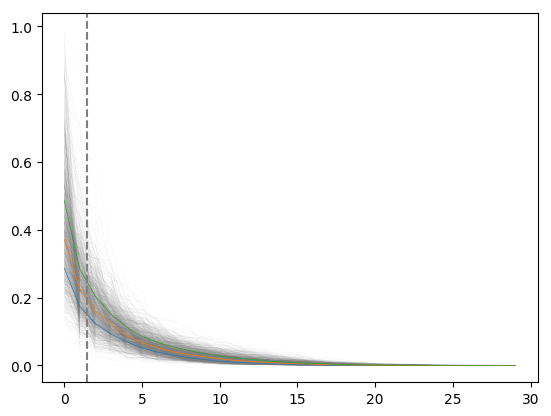
\includegraphics[width=.9\linewidth]{./images/knee.png}
\caption{\label{fig:knee}
\todo{nicer plot on another dataset (this is from RTL)}
Ordered per-label cross-entropy predictions for each example (each grey line) with the median (orange) and IQR (green \& blue) over all examples. Determining a global threshold can be related to visually finding the ``knee'' in that median curve (dotted line).}
\end{figure}


\subsection{Design-algorithm-for-data solutions}
\label{section:background:solution}

In a number of retrieval tasks, a model's out of sample accuracy is measured
on metrics such as AUROC, F1 score, etc. These reflect an objective catered
towards evaluating the model over an entire ranking. Due to the lack of
differentiability, these metrics cannot be directly used as loss functions at
training time (in-sample). A seminal study~\cite{optimizableLosses} derived a
general framework for deriving decomposable surrogates to some of these
metrics. We propose our own decomposable surrogates tailored for the problem
at hand.

With our design-algorithm-for-data approach, we design loss functions that address FIMPUL problems specifically, by optimizing for correct label predictions and correct label count simultaneously.
We first formulate a unified loss, namely
%
\begin{equation}
\label{equation:loss:multilabel}
\underset{\mathcal{L}_{\text {multilabel}}} {\min} \mathcal{F}\left(\cdot ;
\Theta; \mathcal{L}_{\text {multilabel}} (\mathbf{y}, \hat{\mathbf{y}},
\mathbf{n}, \hat{\mathbf{n}}) \right),
\end{equation}
%
Note that although predictions and counts appear explicitly in our Equation~\ref{equation:loss:multilabel},
\(\mathcal{L}_{\text {multilabel}}\) can optimize for both metrics implicitly
(see proposed \emph{sigmoidF1} below). This way, the correlation between label count and label predictions is embedded in the loss. Furthermore, we avoid having to mitigate the importance of label prediction relative to label count with a regularizer $\lambda$. For that purpose, we use surrogates of classical statistical and \ac{IR} metrics.

The proposed design-algorithm-for-data method is thus an alternative to fit-data-to-algorithm and fit-algorithm-to-data. design-algorithm-for-data uses metric as losses, allows for dynamic thresholding and implicitly deals with label counts and label predictions. In the next section, we will detail this approach to derive the \emph{sigmoidF1} loss as a surrogate to optimize for the F1 metric.

% \begin{figure}[t]
% \centering
% 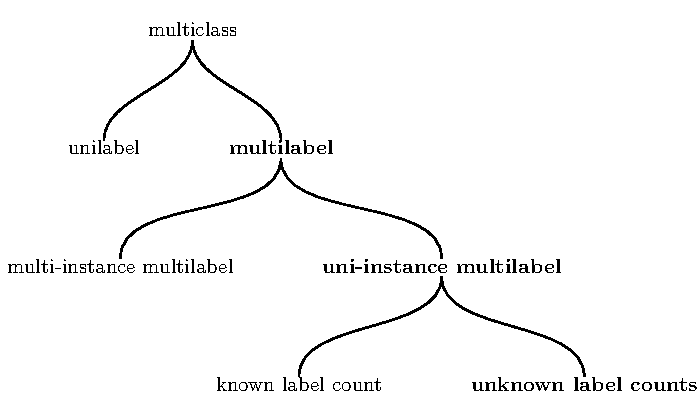
\includegraphics[width=.9\linewidth]{./tree/Tree.pdf}
% \caption{\label{fig:tree} SIMPUL (bold) within the \emph{multiclass}
% nomenclature
% \hvk{figure is not referenced in text, bold is unclear in figure}
% \daan{I think it should go. And if it stays: uni -> single.}
% % Clarifying ``multiclass'' classification problems. In this paper we focus on
% % the uni-instance, multilabel, multiclass classification problem with a
% % varying number of labels (the bottom right hand side of the tree).
% }
% \end{figure}% \mdr{Image source ...}

%%% Local Variables:
%%% mode: latex
%%% TeX-master: "../main"
%%% End: